\chapter{Introduction}
\setcounter{page}{1}
	\section{Narrative}
		\vspace{5mm}
	    \begin{multicols}{2}
		\paragraph{}
			Design patterns are a general re-use solutions to commonly occurring  context problems of software application development.  
			Design patterns typically show the relationships between class instances at run time without specifying the final concrete 
			implementations of the decoupled types.  Furthermore it could be said that Design patterns are the layers between clients and 
			the context of which they are designed to work with while acting as the glue that brings them together in an abstract fashion, 
			allowing them to vary independently.  
			\newline
			\newline
			As part of Software Architectures we were tasked with the project scenario of a game system that implemented design patterns 
			to supported the ‘ilities’ or non functional requirements, some times otherwise known as quality attributes.  Some of these 
			quality attributes include, extensibility, modifiability and modularity and are the primary means of determining software quality.   
			Software architectures which implement these aspirable software characteristics are said to be accomplished via the use of 
			incorporating design patterns into the high level architecture. 
			\newline
			\newline 
			These design patterns are categorized into varieties of creational, structural and behavioral patterns.  As part of the project 
			it was desirable to exhibit these categories through a small subset of the thousands of patterns which make up these categorical 
			hierarchies.   including Observer, Decorator, Strategy, Factory Method, Bridge and one self-researched pattern which we decided 
			upon to be the memento pattern.  These patterns lead into one another  as shown in the diagram derived by the Gang of four, 
			Gamma et al.
			
		\end{multicols}
		
		\begin{figure}[h!]
			\centering
			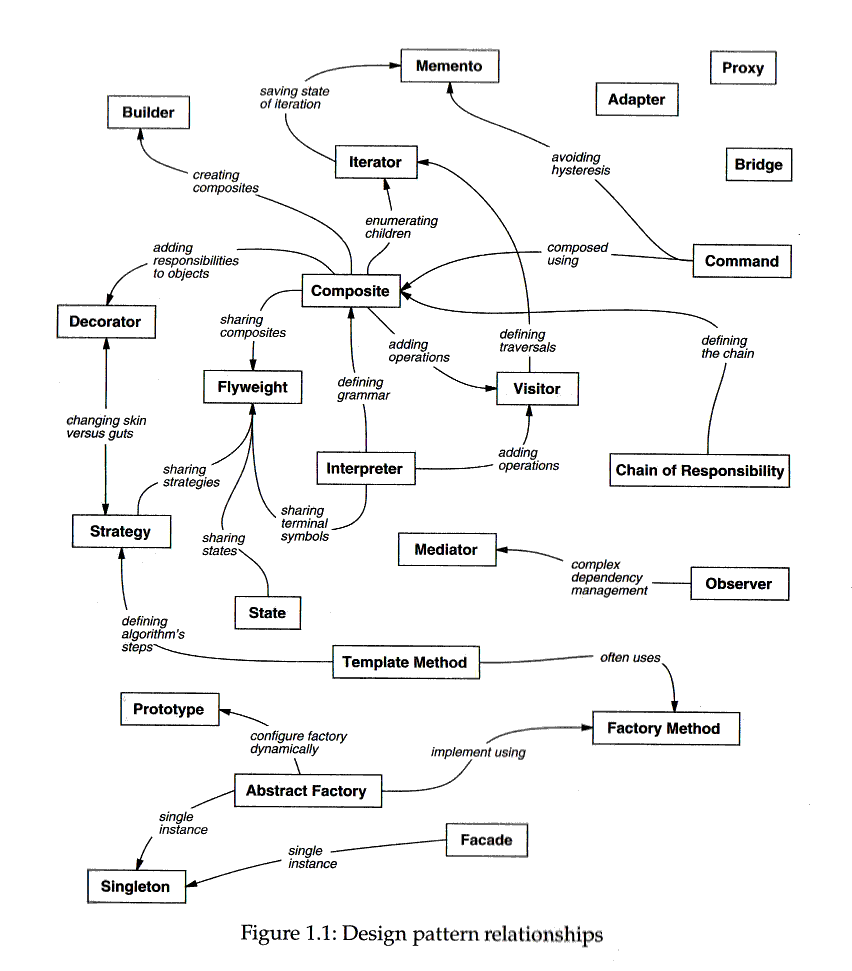
\includegraphics[width=90mm]{figures/DesignPatternRelationships.png}
			  \caption{Gang of four - Pattern Relations}
		\end{figure}
		
		\begin{multicols}{2}
			\paragraph{}
			
			The patterns mentioned above were to implement the run time behaviour, in supporting notifications or events through the system, 
			extending or changing objects as a means to avoid sub classing, behavioural strategies to complete tasks, creational patterns to 
			allow the instantiation of different player types and teams, and the bridge pattern to allow variability between the different 
			visual and text implementations of the game interface.
			\newline
			\newline
			Before any code took place the design was essential to help visual the patterns and the interactions between these patterns 
			and that in of the other supporting patterns in the engine. Visual paradigm was chosen to complete this task.
			\newline
			\newline
			Throughout the development of the system constant refactoring took place to better realise the patterns in the formal sense,  
			refactoring methods such as encapsulate field, generalize type, extract method and extract class where used to decouple and show 
			the cohesive value of the implementation of the patterns.
	    \end{multicols}		
	